\section{Des paires de Cooper dans une cavité à double-dot}
L'expérience consiste à utiliser un nanotube de carbone afin de créer deux puits quantiques de part et d'autre d'une source située au milieu du nanotube.\newline

On peut alors injecter depuis la source des paires de Cooper intriquées, afin d'étudier leur comportement dans un milieu de matière condensée, et la durée de vie de leur intrication.\newline

\begin{figure}[h]
    \begin{center}
        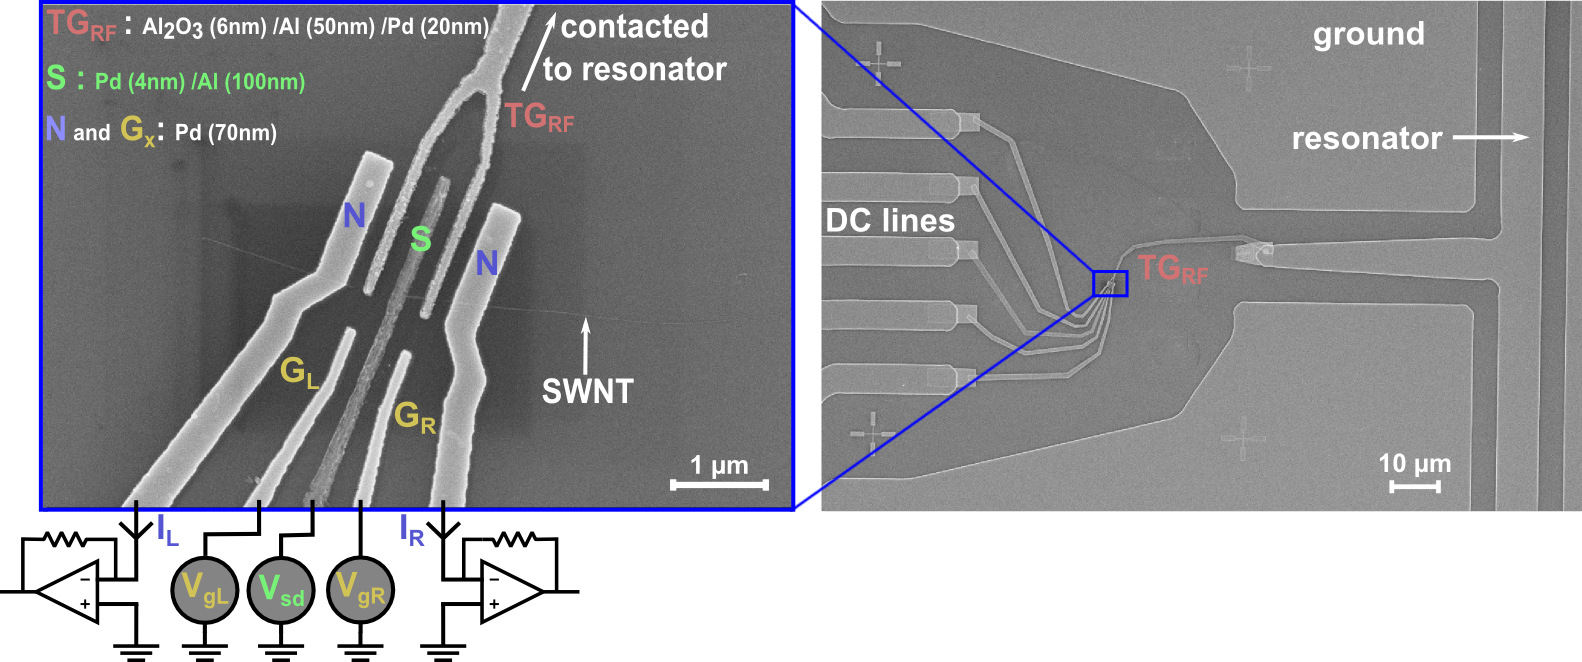
\includegraphics[width=0.8\textwidth]{Images/Expe_photo}
        \caption{Électrodes en contact avec le nanotube de carbone (SWNT)}
        \label{photo_expe}
    \end{center}
\end{figure}

La création des paires de Cooper s'effectue grâce à la nature supraconductrice de l'électrode source : de l'Aluminium.\newline
On remarque sur la photo ci-dessus d'autres électrodes :

\begin{description}
    \item[Les grilles (G$_\text{L/R}$) :] Elles permettent de moduler les potentiels des puits quantiques
    \item[La grille rapide :] Elle relie les grilles au résonateur, dans lequel est envoyé le rayonnement micro-ondes
    \item[Les sorties,] qui permettent de mesurer le courant passé dans chaque puits quantique.
\end{description}


\section{Interactions avec un rayonnement micro-ondes}
On peut, grâce à une ligne HF, envoyer dans la cavité un rayonnement (=photons) autour de 6.65GHz, pour tenter de la faire entrer en résonnance.

La fréquence de résonnance dépend notamment des paramètres des puits quantiques du nanotube de carbone.

On peut alors mesurer les courants I$_\text{L}$,I$_\text{R}$, ainsi que la transmission du résonateur (Amplitude et phase).

\begin{figure}[h]
    \begin{center}
        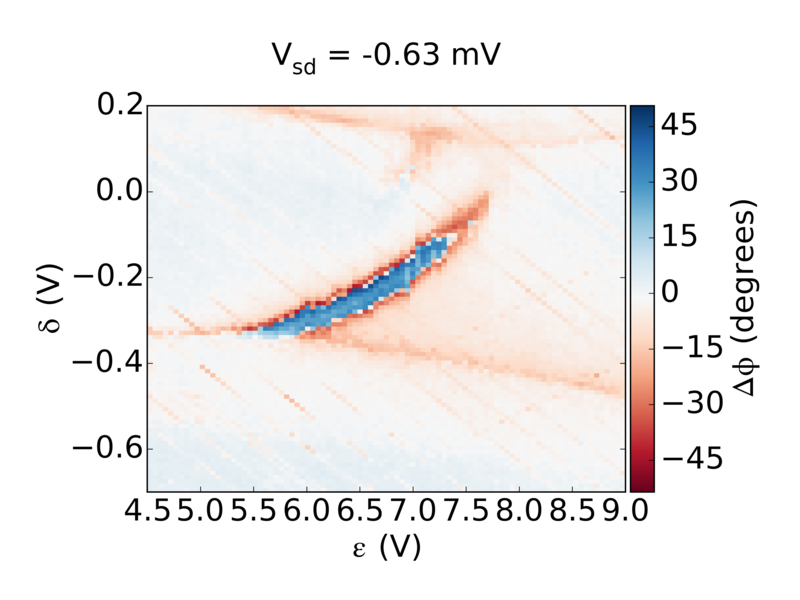
\includegraphics[width=0.4\textwidth]{Images/Sweep/20150422_multigrayscale_DeltaEpsilon_001VsdmV_000__grayscale_phase}
        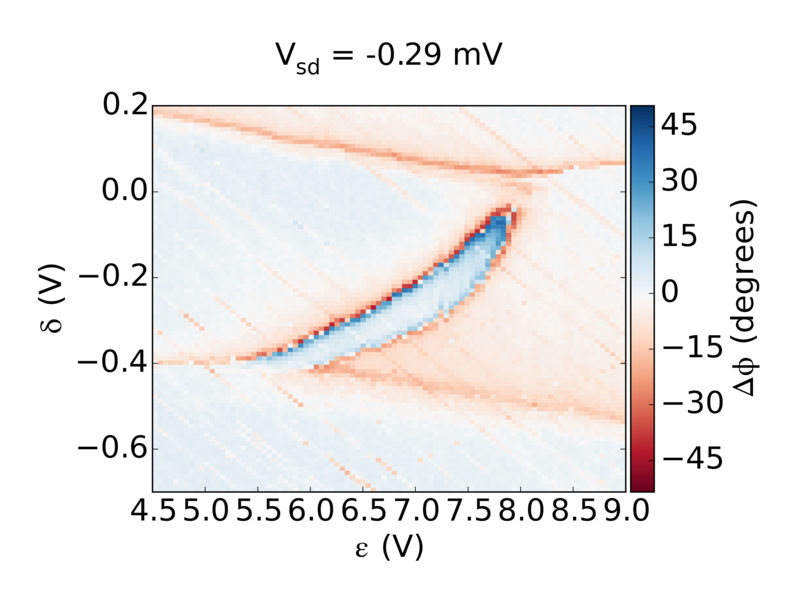
\includegraphics[width=0.4\textwidth]{Images/Sweep/20150422_multigrayscale_DeltaEpsilon_001VsdmV_010__grayscale_phase}
        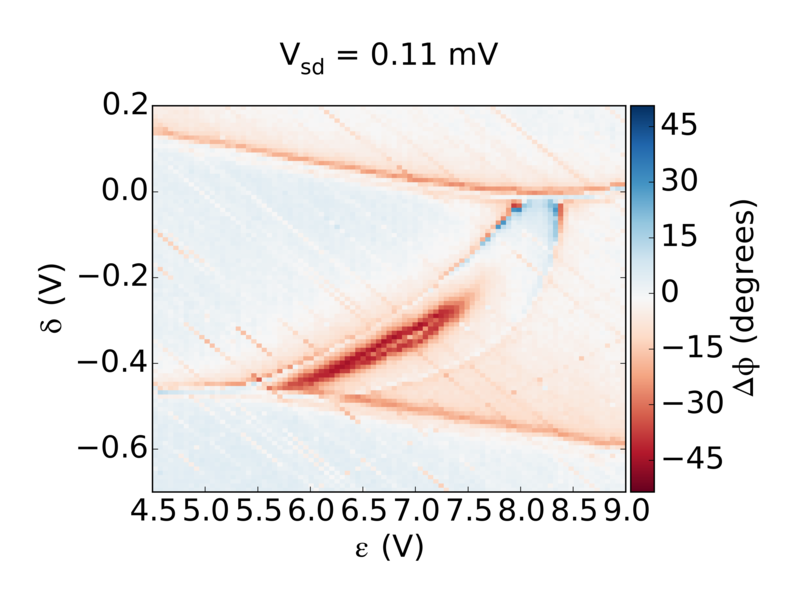
\includegraphics[width=0.4\textwidth]{Images/Sweep/20150422_multigrayscale_DeltaEpsilon_001VsdmV_022__grayscale_phase}
        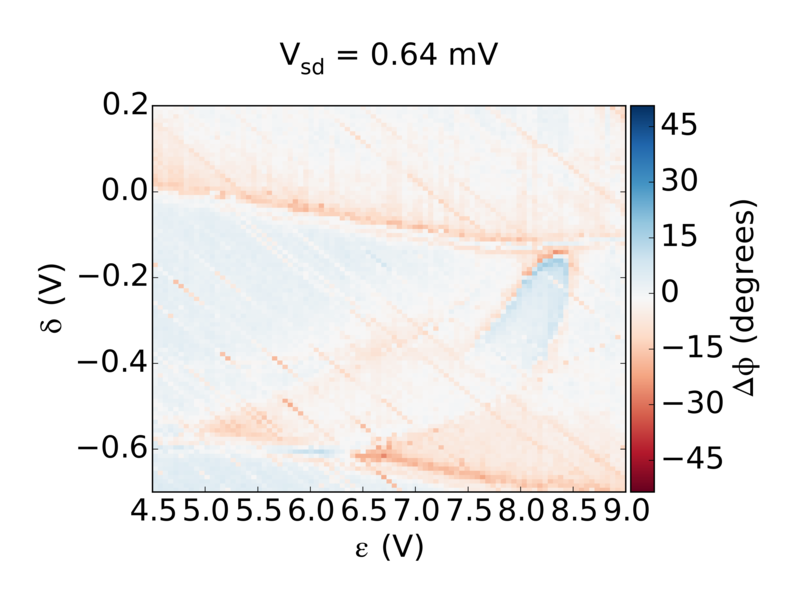
\includegraphics[width=0.4\textwidth]{Images/Sweep/20150422_multigrayscale_DeltaEpsilon_001VsdmV_038__grayscale_phase}
        \caption{Évolution du déphasage induit par le couplage de la cavité au nanotube}
        \label{expe_dephasage}
    \end{center}
\end{figure}

Ici on peut observer un fort changement de phase pour $\varepsilon(V) \uparrow$, ce qui traduit une résonnance du système au niveau de la transition bleu/rouge.\newline

En observant le courant passant dans les sorties dans des conditions similaires, on peut facilement observer un blocage de coulomb :
\begin{figure}[h]
    \begin{center}
        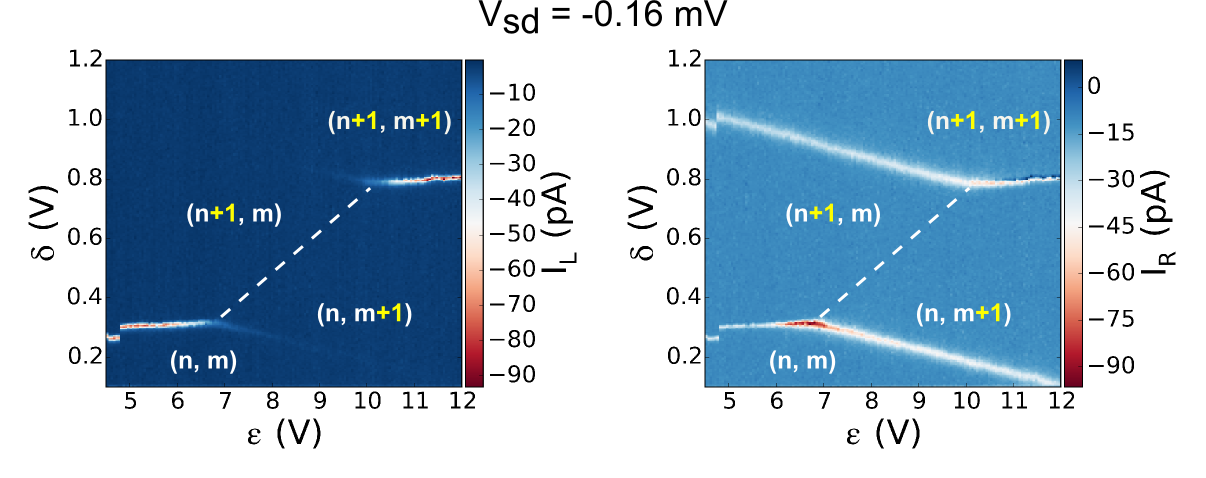
\includegraphics[width=0.85\textwidth]{Images/Exp/CoulombBlockade}
        \caption{Blocage de Coulomb}
        \label{expe_blocagecoulomb}
    \end{center}
\end{figure}

La résonnance entre le rayonnement et la cavité est alors conditionnée par la qualité du rayonnement. C'est pourquoi il faut avoir un contrôle excellent du signal envoyé dans la cavité, et donc des câbles coaxiaux les plus parfaits possibles.


\section{Une cohérence spatiale}
L'hypothèse d'une cohérence spatiale permettant de mesurer du transport quantique à travers le nanotube de carbone repose sur l'absence de bruit ambiant.

Autrement dit, il est nécessaire de placer le système à une température suffisamment faible, et d'empêcher les lignes de signal d'apporter du bruit électronique : une thermalisation excellente des câbles ainsi qu'un rapport signal/bruit suffisant sont nécessaires.\newline

Nous verrons donc plus tard comment nous avons pu obtenir de telles conditions.

\section{Quelques exemples d'expériences}
\subsection{Cooper Pair Splitter}
Elle consiste, comme expliqué plus haut, à étudier le transfert de la source vers les deux sorties des paires de Cooper, en fonction du rayonnement injecté dans la cavité, et inversement la résonnance de la cavité en fonction des paramètres des puits quantiques.

\begin{figure}[h]
    \begin{center}
        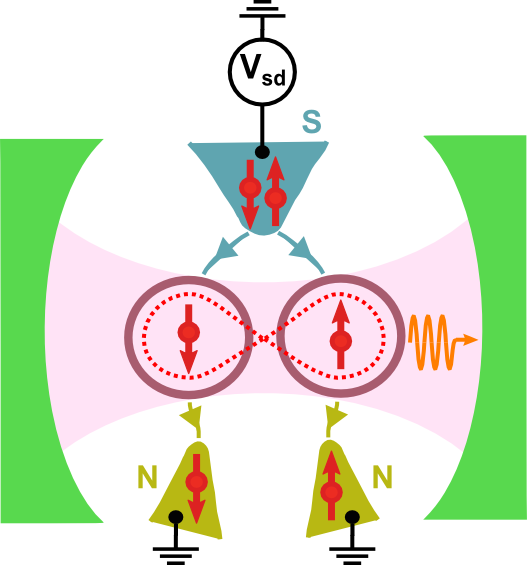
\includegraphics[width=0.50\textwidth]{Images/Exp/Cavity}
        \caption{Représentation du séparateur à paires de Cooper dans la cavité Micro-ondes}
        \label{expe_separateur_dans_cavite}
    \end{center}
\end{figure}

\subsection{Couplage Spin/Trajectoire}
Une autre expérience en cours se dirige vers de l'Électrodynamique Quantique. Elle consiste à appliquer un champ électrique au circuit hybride.

Cela permet alors un couplage fort entre le spin des électrons émis par la source et leur trajectoire. On peut alors discriminer les électrons en fonction de leur spin, grâce aux deux électrodes de sortie.

\subsection{Utilisation du champ magnétique}

La bobine qui a été placée dans le cryostat à dilution pendant mon stage permettra notamment d'appliquer à l'électrode source un champ supérieur à son champ critique supraconducteur : Redevenant métallique, elle ne permet plus de fournir des paires de Cooper intriquées.
\bigskip

\bigskip


Maintenant que le contexte et les contraintes expérimentales ont été exposées, je vais vous présenter les solutions choisies et leur mise en place.
